
\begin{figure*}
	\centering
	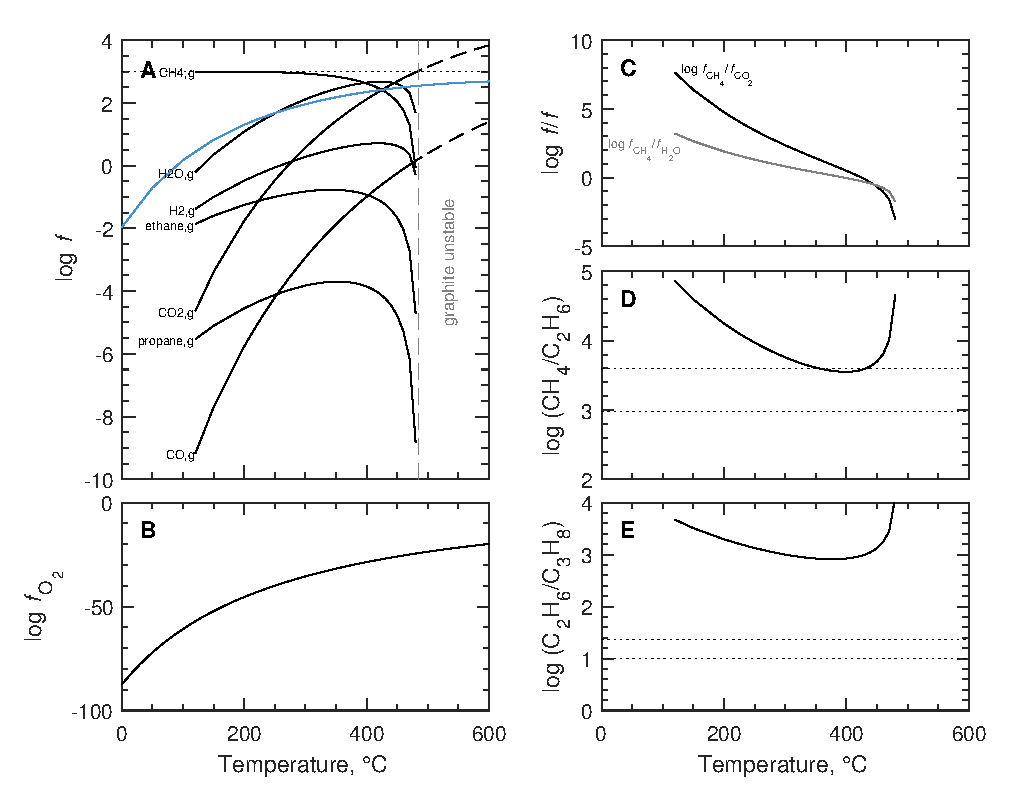
\includegraphics[width=0.95\linewidth]{figures/Fig3.S1}
	\caption[Equilibrium composition of a graphite-saturated C--O--H fluid at 1000~bar with \(f_{\mathrm{O}_{\mathrm{2}}}\) = FMQ]{Equilibrium composition of a
		graphite-saturated C--O--H fluid at 1000~bar (\textbf{A}) with oxygen
		fugacity (\(f_{\mathrm{O}_{\mathrm{2}}}\)) given by the
		fayalite-magnetite-quartz (FMQ) redox buffer (\textbf{B}). The modeled
		fluid is an ideal gas consisting of CO, CO\textsubscript{2},
		H\textsubscript{2}, H\textsubscript{2}O, O\textsubscript{2}, ethane, and
		propane. The model is essentially that of \textcite{French_1966_RG}, with the addition of C\textsubscript{2+} compounds (as also considered by \textcite{Kawagucci++_2013_CG,McDermott_2015_thesis}, with different assumptions regarding redox, water activity, and total mass of carbon). To calculate the
		composition of the fluid, equilibrium constants were computed at various
		temperatures using CHNOSZ \parencite{Dick_2008_GT} from tabulated standard molal
		thermodynamic properties and equation of state parameters \parencite{CHNOSZ_Kel60,CHNOSZ_HDN+78,CHNOSZ_HOK+98,CHNOSZ_WEP+82,Johnson++_1992_CnG,CHNOSZ_Sho93}, the fugacities of CO and CO\textsubscript{2} were
		calculated, and then the fugacities of all other gaseous species were
		solved iteratively under the constraint that $\big\sum\!$\emph{f} = 1000~bar \parencite[a
		pressure typical of those indicated by fluid inclusion studies;][]{Vanko_1988_JGR}. Graphite is unstable above \textasciitilde{}500~°C, as shown
		by the equilibrium fugacities of CO+CO\textsubscript{2} exceeding the
		pressure of the system (dashed lines in A). Ratios of fugacities of
		selected species show that CH\textsubscript{4} is the dominant gas-phase
		species below \textasciitilde{}400~°C (\textbf{C}), and that predicted
		ratios of C\textsubscript{1}/C\textsubscript{2} and
		C\textsubscript{2}/C\textsubscript{3} are
		\textasciitilde{}10\textsuperscript{3} to 10\textsuperscript{4} between
		200 and 400~°C (\textbf{D}, \textbf{E}). Dotted lines in (D) and (E)
		mark the range of C\textsubscript{1}/C\textsubscript{2} and
		C\textsubscript{2}/C\textsubscript{3} measured in hydrothermal fluids
		from the four vent fields we studied \parencite{Charlou++_2000_CG,Charlou++_2002_CG,Proskurowski++_2008_S,McDermott++_2015_PNAS}. The vapor pressure
		curve of water at 1000~bar is shown in blue in (A). Values of
		\(\log f_{\mathrm{H}_{\mathrm{2}}\mathrm{O}}\) that plot above this
		curve are inaccessible because the presence of liquid water sets the
		fugacity of H\textsubscript{2}O and causes the fugacities of
		O\textsubscript{2} and all other species to adjust accordingly.
		Therefore, values of
		\(\log\left({f_{\mathrm{C}\mathrm{H}_{\mathrm{4}}}}\middle/{f_{\mathrm{H}_{\mathrm{2}}\mathrm{O}}}\right) > 0\)
		do not necessarily indicate that total CH\textsubscript{4} content
		exceeds total water content when multiple fluid phases coexist. Liquid
		water has been neglected in our model, but calculations in which
		H\textsubscript{2}O(\emph{l}) is explicitly considered show that
		graphite, an H\textsubscript{2}O-dominated liquid, and a
		CH\textsubscript{4}-rich gas phase can coexist at
		\textasciitilde{}400~°C and \(f_{\mathrm{O}_{\mathrm{2}}}\) close to FMQ
		\parencite{Holloway_1984_G}.}
	\label{fig:3:S1}
\end{figure*}



